\documentclass{standalone}
\usepackage[T1]{fontenc}
\renewcommand*\familydefault{\sfdefault} %%
\usepackage{sfmath}
\usepackage[usenames,dvipsnames]{xcolor}
\usepackage{tikz}
\usepackage{amsmath}
\usepackage{graphicx}
\usepackage{amsfonts}
\usepackage{amssymb}
\usepackage{epstopdf}
\usepackage{pgfplots}
\usepackage{tabularx}
\usepackage{array}

%Information to be included in the title page:
\title{Realistic Intake Rate Scaling Allows For Hyperallometric Fecundity Rate and Later Maturity In Fish}

% \subtitle{Theoretical Ecology}

\author{Luke Vassor \\ \textit{M.Sc. CMEE}}

\date{\today}

\begin{document}


\tikzset{every picture/.style={line width=0.75pt}} %set default line width to 0.75pt        

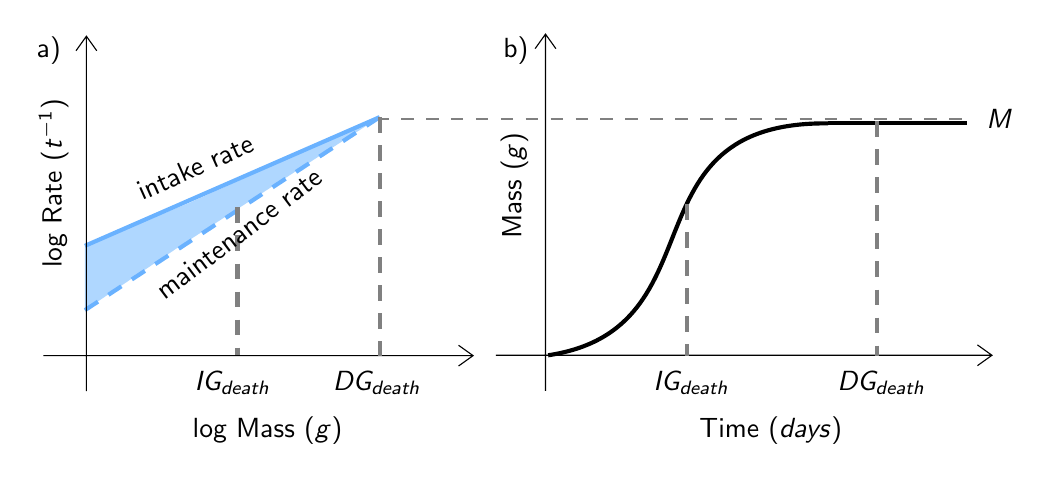
\begin{tikzpicture}[x=0.75pt,y=0.75pt,yscale=-1,xscale=1]
%uncomment if require: \path (0,300); %set diagram left start at 0, and has height of 300

%Shape: Polygon [id:ds6977566036737723] 
\draw  [draw opacity=0][fill={rgb, 255:red, 175; green, 215; blue, 255 }  ,fill opacity=1 ] (166,134) -- (257,93) -- (161,155) -- (115,186) -- (115,155) -- cycle ;
%Shape: Axis 2D [id:dp5730652888146963] 
\draw  (313,207.73) -- (552,207.73)(336.9,53) -- (336.9,224.92) (545,202.73) -- (552,207.73) -- (545,212.73) (331.9,60) -- (336.9,53) -- (341.9,60)  ;
%Curve Lines [id:da13003754679528812] 
\draw [color={rgb, 255:red, 0; green, 0; blue, 0 }  ,draw opacity=1 ][line width=1.5]    (338.15,207.73) .. controls (422.61,195) and (373.1,95) .. (473.09,96) ;


%Straight Lines [id:da7349603249900396] 
\draw [color={rgb, 255:red, 0; green, 0; blue, 0 }  ,draw opacity=1 ][line width=1.5]    (473.09,96) -- (539.81,96) ;


%Straight Lines [id:da8704703169552346] 
\draw [color={rgb, 255:red, 128; green, 128; blue, 128 }  ,draw opacity=1 ][line width=1.5]  [dash pattern={on 5.63pt off 4.5pt}]  (496.6,95) -- (496.6,208) ;


%Straight Lines [id:da8748514340387221] 
\draw [color={rgb, 255:red, 128; green, 128; blue, 128 }  ,draw opacity=1 ][line width=1.5]  [dash pattern={on 5.63pt off 4.5pt}]  (405.13,135) -- (405.13,208) ;


%Straight Lines [id:da5314636216008508] 
\draw [color={rgb, 255:red, 128; green, 128; blue, 128 }  ,draw opacity=1 ][line width=0.75]  [dash pattern={on 4.5pt off 4.5pt}]  (255.36,94) -- (542.09,94) ;


%Straight Lines [id:da6424927530624145] 
\draw [color={rgb, 255:red, 106; green, 178; blue, 255 }  ,draw opacity=1 ][line width=1.5]    (115,155) -- (257,93) ;


%Straight Lines [id:da3232788437561043] 
\draw [color={rgb, 255:red, 106; green, 178; blue, 255 }  ,draw opacity=1 ][line width=1.5]  [dash pattern={on 5.63pt off 4.5pt}]  (115,186) -- (257,93) ;


%Shape: Axis 2D [id:dp6240321433102818] 
\draw  (95,207.9) -- (302,207.9)(115.7,54) -- (115.7,225) (295,202.9) -- (302,207.9) -- (295,212.9) (110.7,61) -- (115.7,54) -- (120.7,61)  ;
%Straight Lines [id:da3156257153648796] 
\draw [color={rgb, 255:red, 128; green, 128; blue, 128 }  ,draw opacity=1 ][line width=1.5]  [dash pattern={on 5.63pt off 4.5pt}]  (188.5,136.5) -- (188.5,207.5) ;


%Straight Lines [id:da5928302189763568] 
\draw [color={rgb, 255:red, 128; green, 128; blue, 128 }  ,draw opacity=1 ][line width=1.5]  [dash pattern={on 5.63pt off 4.5pt}]  (257,93) -- (257,208) ;



% Text Node
\draw (498.65,221) node  [align=left] {$DG_{death}$};
% Text Node
\draw (407.08,221) node  [align=left] {$IG_{death}$};
% Text Node
\draw (445.47,244) node  [align=left] {Time ($days$)};
% Text Node
\draw (555.65,94) node  [align=left] {$M$};
% Text Node
\draw (168,117) node [rotate=-336] [align=left] {intake rate};
% Text Node
\draw (189,149) node [rotate=-323] [align=left] {maintenance rate};
% Text Node
\draw (203,244) node  [align=left] {log Mass ($g$)};
% Text Node
\draw (100,125) node [rotate=-270] [align=left] {log Rate ($t^{-1}$)};
% Text Node
\draw (322,126) node [rotate=-270] [align=left] {Mass ($g$)};
% Text Node
\draw (97.65,61) node  [align=left] {a)};
% Text Node
\draw (322.65,61) node  [align=left] {b)};
% Text Node
\draw (186.08,221) node  [align=left] {$IG_{death}$};
% Text Node
\draw (255.65,221) node  [align=left] {$DG_{death}$};


\end{tikzpicture}


\end{document}